\documentclass[11pt]{article}
\usepackage[T1]{fontenc}
\usepackage[margin=23mm]{geometry}
\usepackage{amsmath,amssymb,booktabs,graphicx,hyperref}
\hypersetup{colorlinks=true,urlcolor=blue,citecolor=blue,
  pdftitle={A 528-chamber counterexample to the octahedral tiling conjecture},
  pdfauthor={Dmitrii Pasechnik}}
\newcommand{\doi}[1]{\href{https://doi.org/#1}{\mbox{doi:\nolinkurl{#1}}}}
\setlength{\parindent}{0pt}
\setlength{\parskip}{5pt}
\title{\Large A 528-chamber counterexample to the octahedral tiling conjecture}
\author{Dmitrii Pasechnik\\[2pt]
  \normalsize Department of Computer Science, Northwestern University}
\date{2026-11-23}
\begin{document}
\maketitle

In the upper half-space model, let \(D_4\) act on the complex boundary plane by multiplication by \(i\) and complex conjugation. Let \(P\) be the hyperbolic convex hull of \(\infty\) and the \(D_4\)-orbits of
\[
0,\quad 1,\quad 2,\quad 1+i,\quad 2+2i,\quad (1+i)/2,\quad (7+i)/5 .
\]
Then \(P\) is an ideal right-angled union of 528 chambers of the SW2 reflection tessellation. It admits no tiling by regular ideal octahedra, even allowing partial face intersections. This gives a counterexample to Conjecture~7.11 of Allcock, Devlin, Felikson, Kontorovich and Whitehead~\cite[\S7.4]{adfkw}. SW2 denotes tetrahedron no.~2 in the Scharlau--Walhorn list~\cite{sw}. We use the face numbering in~\cite[Appendix~B]{adfkw}.

\textbf{Realization.} The 30 ideal points give four vertical facets over the sides of \([-2,2]^2\). The hemispherical facets have the following centers and radii, up to \(D_4\).
\[
\begin{array}{c|ccccc}
\text{center}&2+i&1+i/2&1/2&5/3&5/4\\
\text{radius}&1&1/2&1/2&1/3&1/4\\
\text{multiplicity}&8&8&4&4&4
\end{array}
\]
The facet list follows by taking supporting planes of triples of the ideal points. There are 8 triangles and 24 quadrilaterals. Adjacent hemispheres of radii \(r,r'\) have center distance \(\sqrt{r^2+r'^2}\). A hemisphere adjacent to a vertical facet has its center on the corresponding boundary line. Thus all 60 edges have dihedral angle \(\pi/2\).

Write \(\zeta=z+3+2i\). In these coordinates a hemisphere with center \((a+ib)/d\) and radius \(1/d\) has Lorentz normal \((t,a,b,t-d)\), where \(t=(a^2+b^2+d^2-1)/(2d)\). The displayed circles and the four vertical facets give integral normals of norm one for the form \(-t^2+x^2+y^2+z^2\). Every such normal is conjugate to the simple SW2 normal of face~3. Indeed the simple reflections 1, 3, 4 give signed spatial permutations. Arrange \(x\geq y\geq z\geq0\) after choosing \(t\geq0\). If \(t>0\), the norm equation gives \(t<x+y+z<3t\). The simple reflection in \((1,1,1,1)\) replaces \(t\) by \(2t-x-y-z\), reducing \(\lvert t\rvert\). At \(t=0\) the spatial part is a coordinate unit vector. All facets are therefore SW2 mirrors and \(P\) is a finite union of chambers. Chamber adjacency enumeration gives 528. Let \(W\) be the SW2 reflection group and \(H\) the subgroup generated by the 32 facet reflections of \(P\). As an independent check, Todd--Coxeter coset enumeration~\cite{tc} in GAP~\cite{gap} gives \([W:H]=528\).

\textbf{Why boundary edges force tiles.} Every ideal vertex of a contained tile is a cusp of \(P\), by strict convexity of the unit ball in the Klein model. At an ordinary point of a boundary edge of \(P\), both supporting planes support any tile containing that point. The point must be on a tile edge, since tile vertices are ideal. The entire edge has the same two ideal endpoints and the tile fills the right angle. Its two incident triangular faces consequently lie in the two supporting planes of \(P\).

\newpage
\textbf{Two incompatible octahedra.} For \(s=1,2\) write \(O_s\) for the regular ideal octahedron with vertices \(\infty,0,s,is,s+is,s(1+i)/2\). The edge \(e_2=(2+2i,2)\) forces \(O_2\). The edge \(e_1=(1,(1+i)/2)\) forces \(O_1\).

To check the first assertion, use the quadrilateral facet with vertices \(\infty,2+2i,2,2-2i\). For the second use the one with vertices \(0,1,(1+i)/2,(1-i)/2\). The third vertex \(c\) of the triangular tile face must be one of the other two cusps in the indicated quadrilateral. Each triangle has precisely two octahedral completions. In the table an entry in parentheses gives a required cusp absent from \(P\).

\begin{center}
\begin{tabular}{cccc}
\toprule
Edge & Third cusp \(c\) & First completion & Second completion\\
\midrule
\(e_2\) & \(\infty\) & \((3+i)\) & \(O_2\)\\
\(e_2\) & \(2-2i\) & \(((14+2i)/5)\) & \(((6+2i)/5)\)\\
\(e_1\) & \(0\) & \((1/2)\) & \(O_1\)\\
\(e_1\) & \((1-i)/2\) & \((1/2)\) & \(((3+i)/2)\)\\
\bottomrule
\end{tabular}
\end{center}

The entries follow by taking the M\"obius map \(M\) sending \(0,\infty,1\) to the ordered edge endpoints and \(c\). The three remaining vertices are \(M(\pm i)\), \(M(1\pm i)\), and \(M((1\pm i)/2)\), with signs chosen consistently.

On a sufficiently high horosphere at \(\infty\), the sections of \(O_2\) and \(O_1\) are \([0,2]^2\) and \([0,1]^2\). The point above \((1/2,1/2)\) at height 3 is strictly inside both tiles. Their interiors overlap, proving the assertion.

\begin{center}
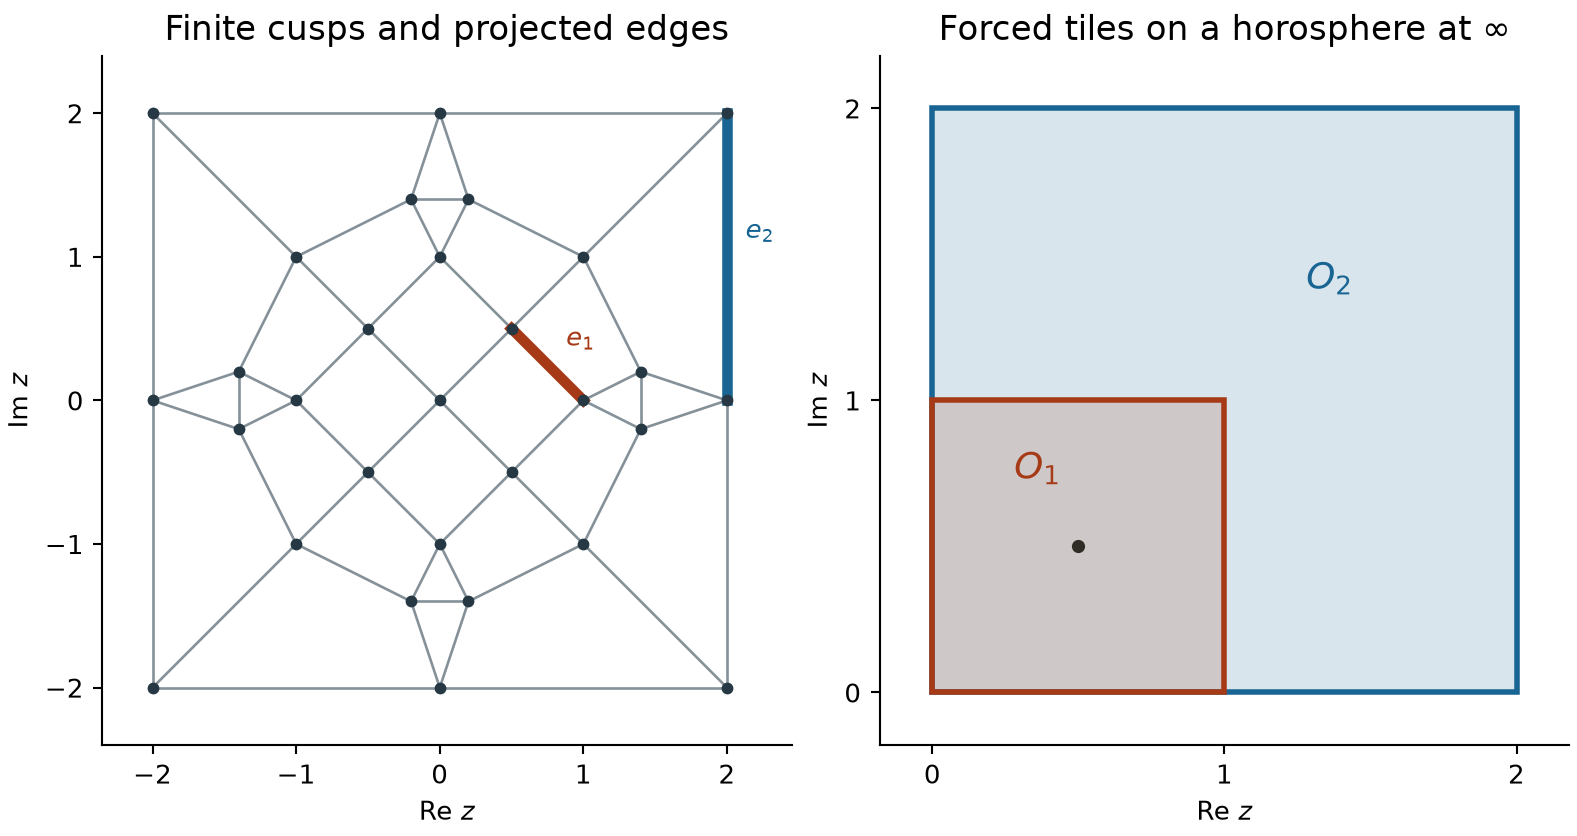
\includegraphics[width=.97\linewidth]{counterexample-528.png}
\end{center}
An independent enumeration of all six-point octahedral placements finds 27. The boundary edges force 12 distinct tiles while the hyperbolic volume of \(P\) is exactly eleven octahedra.

\newpage
\section*{Computational details}
An initial census in Julia~\cite{julia} enumerated small unions of SW2 chambers. The search that found \(P\) used Python~\cite{python}. With one cusp at infinity, it fixed the four vertical walls and enumerated hemispherical mirrors of bounded curvature. The accompanying script \texttt{counterexample.py} reconstructs \(P\) from the seven cusp representatives and checks the obstruction in exact arithmetic. The file \texttt{results/counterexample-528.g} gives the 32 facet reflections as words in the generators of \(W\). The figure was drawn with Matplotlib~\cite{matplotlib}.

An auxiliary calculation in \texttt{coxeter\_checks.g} used HAP~\cite{hap} to construct the Davis complex of the ambient group \(W\) from its Coxeter matrix. In the simplicial model of this contractible \(W\)-space~\cite{davis,davis-book}, a simplex is a chain of cosets of finite standard parabolic subgroups, ordered by inclusion. The \texttt{DavisComplex} routine of Rahm and S\'anchez-Garc\'ia~\cite{hap-davis,sg} gives \(14,43,48,18\) orbits of simplices in dimensions \(0,1,2,3\), respectively.

\paragraph{Acknowledgment.}
I used OpenAI Codex~\cite{codex} to develop and run the search and verification programs, identify the two forced octahedra, and draft the proof and this note.

\begin{thebibliography}{99}
\small\raggedright
\setlength{\itemsep}{2pt}

\bibitem{adfkw} D. Allcock, P. Devlin, A. Felikson, A. Kontorovich and I. Whitehead.
\emph{Arithmetic Polyhedra}. Preprint, 4 September 2026.
\href{https://arxiv.org/abs/2609.05349v1}{arXiv:2609.05349v1 [math.MG]}.

\bibitem{julia} J. Bezanson, A. Edelman, S. Karpinski and V. B. Shah.
Julia: A fresh approach to numerical computing. \emph{SIAM Review} \textbf{59} (2017), 65--98. \doi{10.1137/141000671}.

\bibitem{davis} M. W. Davis. Groups generated by reflections and aspherical manifolds not covered by Euclidean space. \emph{Ann. of Math.} (2) \textbf{117} (1983), 293--324. \doi{10.2307/2007079}.

\bibitem{davis-book} M. W. Davis. \emph{The Geometry and Topology of Coxeter Groups}.
Second edition, Springer, 2025. \doi{10.1007/978-3-031-91303-7}.

\bibitem{hap} G. Ellis. \emph{HAP, Homological Algebra Programming}.
GAP package, version 1.79, 2026. \mbox{\url{https://gap-packages.github.io/hap/}}.

\bibitem{gap} The GAP Group. \emph{GAP -- Groups, Algorithms, and Programming}.
Version 4.16.1, 2026. \mbox{\url{https://www.gap-system.org/}}.

\bibitem{matplotlib} J. D. Hunter. Matplotlib: A 2D graphics environment.
\emph{Computing in Science \& Engineering} \textbf{9} (2007), no.~3, 90--95. \doi{10.1109/MCSE.2007.55}.

\bibitem{codex} OpenAI. \emph{Codex}. Software, used November 2026. \mbox{\url{https://openai.com/codex/}}.

\bibitem{python} Python Software Foundation. \emph{The Python Language Reference}.
Python 3.14. \mbox{\url{https://docs.python.org/3.14/reference/}}.

\bibitem{hap-davis} A. D. Rahm and R. J. S\'anchez-Garc\'ia. \emph{Davis Complex}.
HAP subpackage and documentation. \href{https://gaati.org/rahm/subpackage-documentation/aboutDavisComplex.html}{Implementation and examples}.

\bibitem{sg} R. J. S\'anchez-Garc\'ia. Equivariant \(K\)-homology for some Coxeter groups.
\emph{J. London Math. Soc.} (2) \textbf{75} (2007), 773--790. \doi{10.1112/jlms/jdm035}.

\bibitem{sw} R. Scharlau and C. Walhorn. Integral lattices and hyperbolic reflection groups.
\emph{Ast\'erisque} \textbf{209} (1992), 279--291. \href{https://numdam.org/book-part/AST_1992__209__279_0/}{Numdam}.

\bibitem{tc} J. A. Todd and H. S. M. Coxeter. A practical method for enumerating cosets of a finite abstract group.
\emph{Proc. Edinburgh Math. Soc.} (2) \textbf{5} (1936), 26--34. \doi{10.1017/S0013091500008221}.
\end{thebibliography}
\end{document}
